\lab{Algorithm}{Line Sweep}{Line Sweep}

\objective{Learn about and implement a basic line sweep algorithm}

\section*{General Line Sweep Algorithms}

Line sweep algorithms are a significant group of algorithms with a variety of applications. 
In the strictest sense, line sweep algorithms typically use a priority queue and binary tree to lower the temporal complexity associated with certain tasks. 
Some notable examples include Fortune's Algorithm for calculating Voronoi diagrams and Andrew's Algorithm for computing the convex hull of a set of points. 
In this lab, we will explore a basic line sweep algorithm that allows efficient computation of the Closest Pair problem.  Given a set of points, find the distance between the closest pair of points.

\section*{Na\"ive Implementation}

The obvious way of doing this is to simply compute the distance between each point and each of the other points.
However, this requires $n^2$ computations where $n$ is the number of points (10 points requires calculating 100 distances).
Since distance is symmetrical, we can compare each point with the points that follow it in the list we are given (which will reduce
the total number of distances to be computed).
A good implementation is as follows:
\begin{lstlisting}
def multidist(p0,p1):
    l=len(p0)
    return sum([(p0[i]-p1[i])**2 for i in range(l)]**.5
def badmindist(X):
    l=len(X)
    r=multidist(X[0],X[1])
    for i in xrange(l):
        for j in xrange(i+1,l):
            d=multidist(X[i],X[j])
            if d<r:
                r=d
    return r
\end{lstlisting}

Since, on average, we iterate through half the list per point added, this algorithm will have complexity $O(n^2)$ (we are only scaling by a constant factor).  It is faster than the truly na\"ive method, but essentially just as inefficient.
For very small numbers of points, this algorithm works, but it quickly becomes inefficient for all but the smallest numbers of points.  What we would like to do is go from $n^2$ to something better.  To do this, we have to think about the problem differently.
We introduce the line sweep algorithm which is one of the key techniques of computational geometry.

\section*{A Simplified Line Sweep Algorithm}

The concept behind a line sweep algorithm is breaking a global problem into a sequence of
problems that can be solved locally.  We sweep the domain space with a line.
This line divides the domain space into an explored region and an unexplored region.
As the line sweeps, events occur, be it whether the line encounters a point in the data set
or some other type of event.  We compute the solution at the very beginning of the line sweep
and as new events happen, we compute the change that these events have on our current solution.
We only need to consider the events in the explored region or on the sweep line as they are the
only events that affect the current solution.  Sweep line algorithms typically exhibit a temporal
complexity of $O(n \log n)$, far better than $O(n^2)$.

Line sweep algorithms are helpful for doing all sorts of proximity based computations.
In the example above, we took advantage of the fact that distance was symmetric ($d(a,b)=d(b,a)$).
In a line sweep version of this algorithm, we also take advantage of the fact that any points further
than the current smallest minimum distance do not need to be considered.  The secret to
the line sweep solution for the closest pair problem is to actually have two sweep lines that have
some constant distance between them.  When computing distances between points, we only need to consider
the points that lie between the two sweep lines.  Because of this, it is clear to see that we would want
the distance between the sweep lines to be equal to the current minimum distance we have computed.
This eliminates all points with distances from the current point greater than the minimum distance.

For a general line sweep algorithm, it is common to use a priority queue to order the items that need to be processed.
We have implemented a very basic priority queue in the file \li{pqueue.py}. 
A more complex priority queue can be found in the library \li{Queue} that is included in Python. 
The points can be added into the queue by using the \li{add(data,priority)} method for the priority queue object. 
You can get the next item in the priority queue using the \li{get()} method. 
In this case you will want to add points into the queue with priority equal to their $x$-value. 
If their $x$-values are equal, they will be returned in the order they are entered. 
You could give a tuple for the order of the point, then the queue would order them by $x$ value and then, when $x$ values are equal, by $y$ value, but that is more expensive computationally and it makes no difference in the actual implementation of the algorithm. 

We track the points in the area between the two sweep lines with a list.  Many line sweep algorithms like to use a binary tree
to do this because of the fast insert and search times.  We, instead, use a list combined with a binary search.  Each time we advance
the sweep lines, we update this list so it always contains the points between the sweep lines (adding or removing points where necessary).
A point stays in the list if its distance from the front sweep line is less than the current minimum distance.

Assuming we have already ordered all our points by $x$ coordinate, we can perform the line sweep as follows.
\begin{enumerate}
\item Process the first two points and add them to the active list.
Set current minimum distance to the distance between these two points.
\item Get the next point in the priority queue.
\item Update the active list containing the points between the two sweep lines.
\item Compute the distance between the current point and all the points in the active list.
Compare the smallest distance with the current minimum distance.
\item Repeat steps 2 to 5 for all remaining points in the priority queue
\end{enumerate}
When the algorithm terminates, the current minimum distance will the be distance between the closest pair of points.

This algorithm can be illustrated as follows:
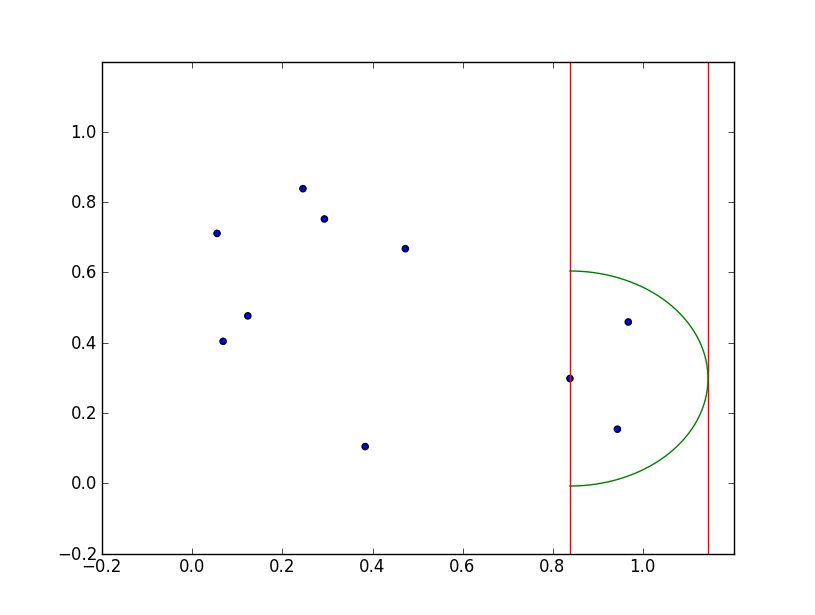
\includegraphics[width = \textwidth]{simple1.png}
After processing the first two points, we process the third point and see that our minimum distance thus far has dropped.

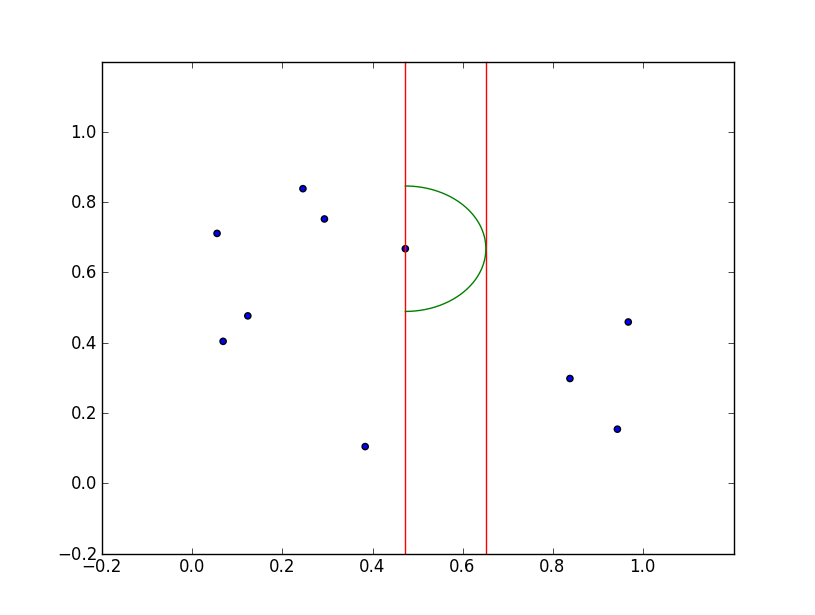
\includegraphics[width = \textwidth]{simple2.png}
This change in the minimum thus far is reflected in how we form the actives list for the next point we process. 
We remove the points from the top of the queue that are too far away in the $x$ direction to have a distance less than the current minimum. 
We then process anything that is left.

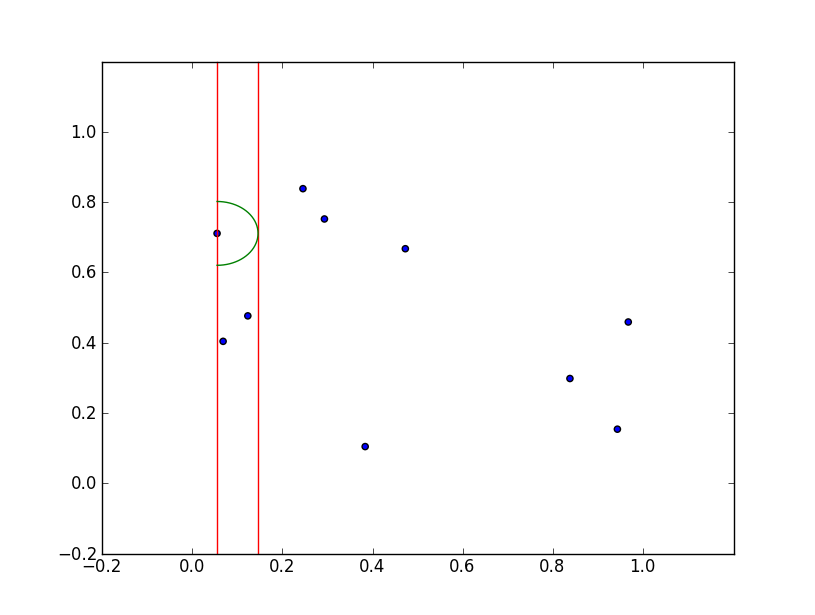
\includegraphics[width = \textwidth]{simple8.png}
After iterating over all the points in the set, we have the final minimum distance desired.

\begin{problem}
Implement the above line sweep algorithm for finding the closest pair of points in a set of points.
\end{problem}

\begin{problem}
You may have noticed that, in this closest pair problem, the priority queue is only used to sort the points passed to the function. 
Sorting the points can be done more quickly using array operations. 
%This is not always the case with general line sweep algorithms. 
Write a version of the function which copies the array and sorts the copy in place. 
Something like \li{X=Y[Y[:,0].argsort()]} will do this for you. 
Note that the sorted version will be sorted from smallest to largest and not largest to smallest, so you will have to make appropriate changes in your implementation.
Make sure your new function works in arbitrary dimensions. 
Modify the code so that it will accept a metric function as a parameter.
This metric function should take a point and an array of points as arguments and return an array of distances from the point to each of the points in the array. 
Test your function's speed. 
How does it scale as you increase the number of points? 
How does it scale as you increase the number of dimensions?
\end{problem}

\section*{A Line Sweep Algorithm}

You may have noticed that we are not exploiting all of the symmetry of the problem in the previous algorithm. 
It would likely speed things up if we could also slice away the points that have $y$ values that could not possibly yield the minimum distance. 
The list operations involved in doing this are somewhat more involved. 
As it turns out, it is easier to implement this line sweep by sorting the points by $y$ value, then slicing our actives list by $x$ value.
In order to slice the list efficiently, we will need to order our active points with respect to their $y$ values, but continue to remove them according to their $x$ value. 
There are a variety of ways this can be done. 
Many line sweep algorithms would use a binary tree to store these points and get good insertion and deletion times. 
This is doable, but in this case, except for very poorly conditioned problems, our actives list tends to remain small, so we can do this with a list. 

To do this insertion, we will use a binary search over the list. 
The functions \li{bisect_left} and \li{bisect_right} from the \li{bisect} module will do this for you. 
A binary search over a list works under the assumption that the list is already ordered and gives you a fast way to know where to insert an item in your ordered list. 
At each iteration, we will first remove the points that no longer are important to the points we are processing. 
We will then iterate only over the pertinent part of the actives list, according to the range of $x$ values that are close to the point we are processing.

% For speed, when updating the active list, you should modify the list in place. 
% What this means is that instead of removing each point individually as you iterate over the list, you should do something like \li{actives[:] = [p for p in actives if (p[1] - y) <= r]} 
% Using a list comprehension in this way allows you to filter out the points you need to remove without so many repeated list operations. 

You should use a binary search to figure out where you need to cut your list. 

Also, for large numbers of points, you will want to import the functions you call into the local namespace to save on lookup time. 
For each function, you can do this using a line of code that is something like \li{_bl = bs.bisect_left}. 

This algorithm can be illustrated as follows:

Note: in this case we sweep along the $x$ axis from right to left.

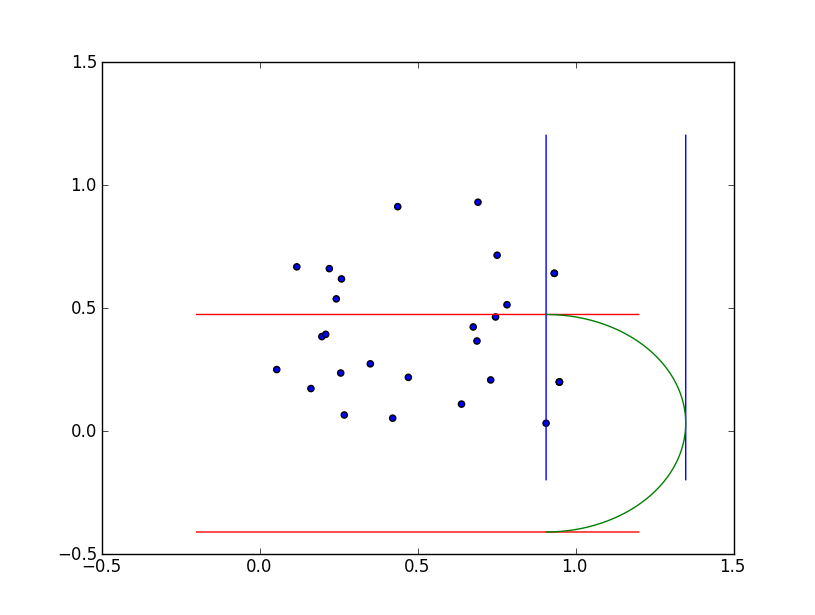
\includegraphics[width = \textwidth]{ptsweep1.png}
In processing the first point, we find find that we must reduce the radius. Notice that we only need to consider the points that lie in the box formed by the red an blue lines.


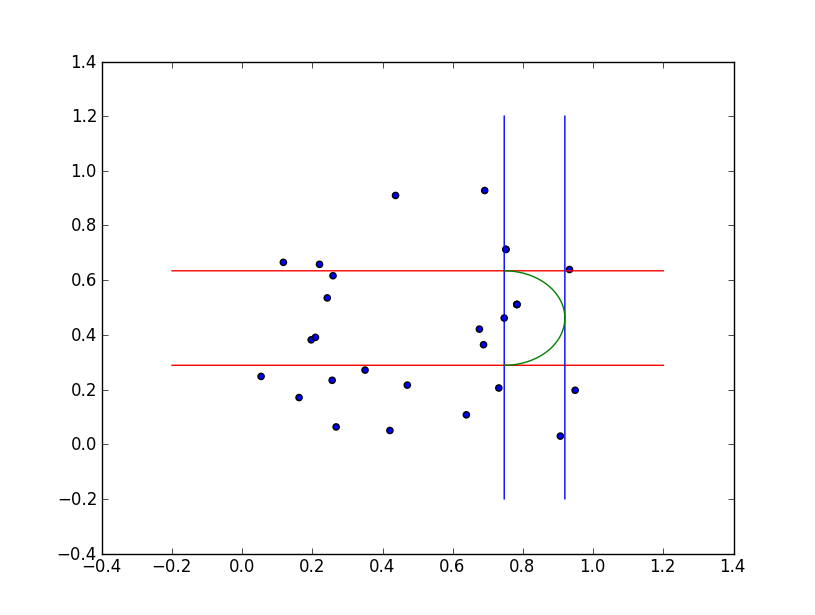
\includegraphics[width = \textwidth]{ptsweep4.png}
A few more points along, we find that we mus reduce our minimum radius significantly.

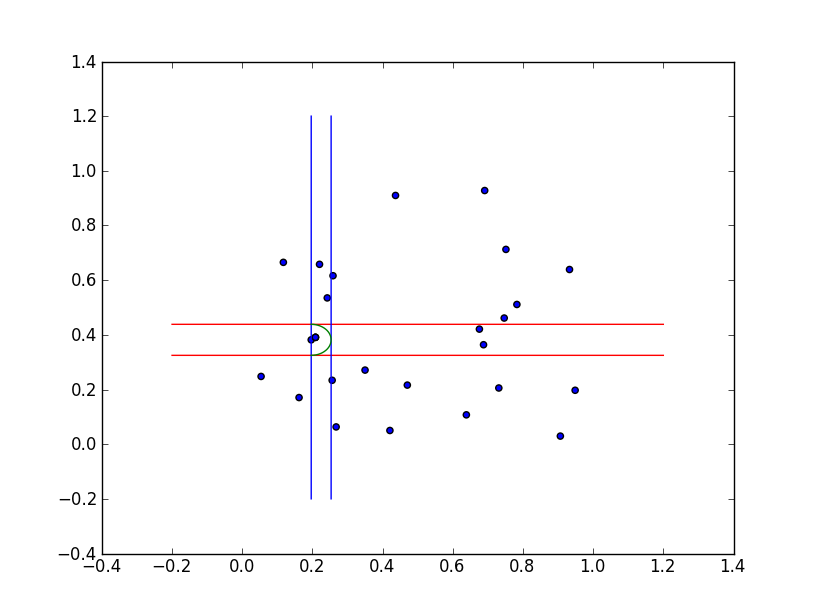
\includegraphics[width = \textwidth]{ptsweep20.png}
This is where we actually hit the minimum distance.

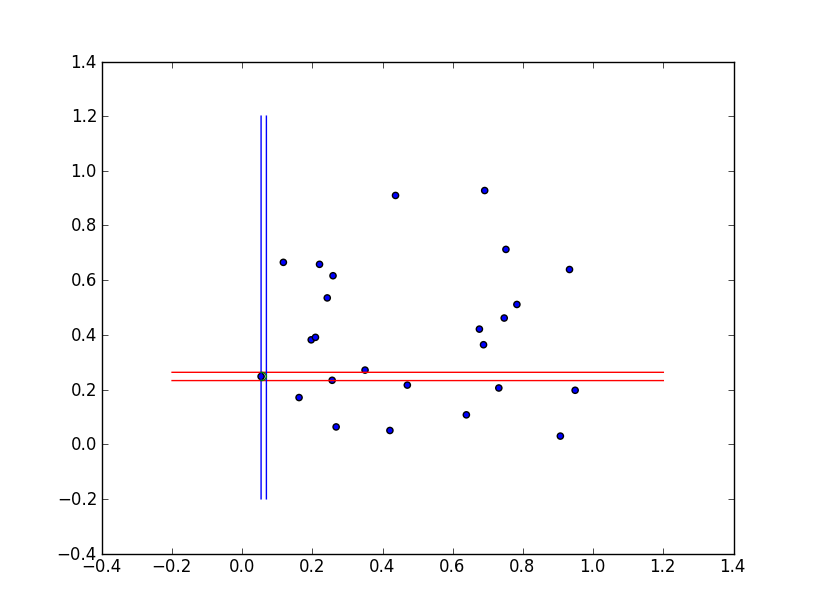
\includegraphics[width = \textwidth]{ptsweep23.png}
After processing through all the points, we are guaranteed to have hit the minimum distance already, so our minimum distance thus far is our final return value.

\begin{problem}
Implement the algorithm above in 2 dimensions. 
Time it against the naive implementation at the beginning of this lab and against the simplified version you coded above.
The new version should be faster, but speed depends heavily on how you have implemented it, so you may have some optimization left to do.
\end{problem}

\begin{problem}
Write a different version of the algorithm above which masks arrays to eliminate the points that do not need to be processed. 
Use recursion to mask over arbitrarily many dimensions. 
Allow the user to input a metric function like you did with the simpler version.
Compare the speeds of your implementations on different data sets.
Note: you may want to sort the points by $x$ value for this version.
\end{problem}

There are a variety of ways this algorithm can be implemented, and the actual performance for a real world problem will depend on your ability to exploit the symmetry of the situation at hand. 
Theoretically, the best way to do this is to use a binary search tree to store the list of active points, but initial cost of using these objects is expensive and outweighs the benefits in Python.
Practically speaking, Python is designed for easy programming and high programmer output, so many of the details of how fast something will run depend on the details of how all the different objects used have been implemented.
To fully speed up a Python function, you would want to use an efficient algorithm, try several implementations, and use Cython or some lower level language to perform optimizations wherever possible. The fastest implementations are likely to be written in lower level languages.